\documentclass[]{llncs}

\usepackage{graphicx}
% Used for displaying a sample figure. If possible, figure files should
% be included in EPS format.
%
% If you use the hyperref package, please uncomment the following line
% to display URLs in blue roman font according to Springer's eBook style:
% \renewcommand\UrlFont{\color{blue}\rmfamily}

% Display polish characters
\usepackage[polish]{babel}
\usepackage[utf8]{inputenc}

% Translate some names to polish
\def\keywordname{{\bf Słowa Kluczowe:}}

\begin{document}

\title{Wykorzystanie Ethereum do Budowy Zdecentralizowanej Aplikacji}
\author{Wojciech Korzeniowski}
\institute{
  Instytut Informatyki\\Wydział Elektroniki i Technik Informacyjnych\\Politechnika Warszawska\\
  \url{http://www.ii.pw.edu.pl/}
}

\maketitle

\begin{abstract}

  Opis zdecentralizowanej aplikacji zbudowanej zbudowanej na platformie Ethereum
  z wykorzystaniem smartkontraktów Ethereum\cite{ethereum}.
  \keywords{Smart contract \and Blockchain \and DApp}

\end{abstract}

\section{First Section}
\subsection{Second Section}
\subsubsection{Third Section}
\paragraph{Fourth Level}
Lorem ipsum dolor sit amet, consectetur adipiscing elit.


%
% ---- Bibliography ----
%
% BibTeX users should specify bibliography style 'splncs04'.
% References will then be sorted and formatted in the correct style.
%
% \bibliographystyle{splncs04}
% \bibliography{mybibliography}
%
\begin{thebibliography}{8}
  \bibitem{ethereum} Ethereum Homepage, \url{https://www.ethereum.org/}
\end{thebibliography}



% ########## START OF SAMPLES

\newpage
\newpage

\section{Takie tam przydatne przykłady}
\begin{definition} text \end{definition}
\begin{case} text \end{case}
\begin{proof} text \end{proof}

\noindent Widać na równaniu:
\begin{equation}
  x + y = z
\end{equation}

Please try to avoid rasterized images for line-art diagrams and
schemas. Whenever possible, use vector graphics instead (see
Fig.~\ref{fig1}).

\begin{figure}
  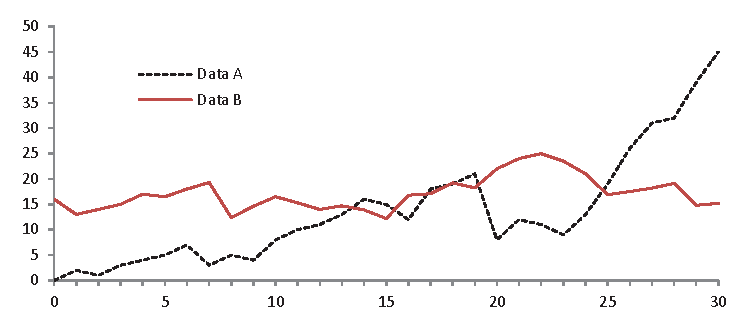
\includegraphics[width=\textwidth]{fig1.eps}
  \caption{A figure caption is always placed below the illustration.
    Please note that short captions are centered, while long ones are
  justified by the macro package automatically.} \label{fig1}
\end{figure}

Tabla~\ref{tab1} przedstawia że działa.

\begin{table}
  \caption{Table captions should be placed above the
  tables.}\label{tab1}
  \begin{tabular}{|l|l|l|}
    \hline
    Heading level &  Example & Font size and style\\
    \hline
    Title (centered) &  {\Large\bfseries Lecture Notes} & 14 point, bold\\
    1st-level heading &  {\large\bfseries 1 Introduction} & 12 point, bold\\
    2nd-level heading & {\bfseries 2.1 Printing Area} & 10 point, bold\\
    3rd-level heading & {\bfseries Run-in Heading in Bold.} Text follows & 10 point, bold\\
    4th-level heading & {\itshape Lowest Level Heading.} Text follows & 10 point, italic\\
    \hline
  \end{tabular}
\end{table}

% ########## END OF SAMPLES

\end{document}
